\chapter{LFS-Facebook}

\section{Progetti di partenza}
Una fase preliminare del tirocinio è stata impiegata principalmente nello studio di due progetti open source: LFS e django-facebook.

LFS è un negozio online che  si basa su Python, Django(Web framework per Python) e jQuery. A questo è stato aggiunto poi un tema responsivo (anch'esso basato su un altro progetto open-source, bootstrap), ed il tutto ha rappresentato la base sulla quale aggiungere delle funzionalità legate principalmente alla sua integrazione come applicazione fruibile su Facebook. 

Django-facebook, invece, permette ad applicazioni django di registrare gli utenti tramite backend Facebook, convertendo i dati ricevuti dall'operazione di log in con Facebook, in un modello consono alle modalità di storing attraverso django.

\section{Gestione backend di autenticazione}
Un'esigenza che un progetto di un'applicazione potrebbe avere è quella di dover/voler pescare da un'altra sorgente di usernames e passwords.

Questo è proprio il nostro caso, vogliamo usare come backend di autenticazione quello di Facebook.
Per iniziare si è testata un'applicazione django come LFS con LDAP. 

LDAP è un protocollo di livello applicativo per accedere e gestire servizi di directory su una rete IP. Uno degli usi più comuni di LDAP è quello di fornire un “single sign-on” dove per la coppia d'informazioni utente:password è condivisa tra diversi servizi.
Nel nostro caso è stato utilizzato openLDAP, un'implementazione opensource del suddetto protocollo.

Per aggiungere questa funzionalità ad un'applicazione Django è necessario modificare la variabile AUTHENTICATION BACKENDS del file setting.py, in particolare Django mantiene una lista di “authentication backends” che egli verifica per ogni autenticazione. 

Quando qualcuno cerca di autenticarsi, Django prova l'autenticazione lungo tutta la lista di backend per cui è impostato. 
Attenzione che l'ordine è importante in quanto django si fermerà al primo match positivo.

Per quanto riguardo openLDAP sono necessarie anche tutta un'altra serie di impostazioni da specificare per l'accesso al server, e la ricerca; qui un esempio di configurazione minimale:
\begin{lstlisting}
AUTH_LDAP_SERVER_URI = "ldap://ldap.example.com"

AUTH_LDAP_BIND_DN = "cn=django-agent,dc=example,dc=com"
AUTH_LDAP_BIND_PASSWORD = "phlebotinum"
AUTH_LDAP_USER_SEARCH = LDAPSearch("ou=users,dc=example,dc=com",
    ldap.SCOPE_SUBTREE, "(uid=%(user)s)")
\end{lstlisting}
vengono così configurate  due operazioni fondamentali: Bind, che esegue l'autenticazione, e Search che esegue una ricerca. Nella struttura ad albero, ad ogni livello esiste un Relative distinguished name (RDN) che lo identifica (ad esempio ou=people). L'unione di tutti i RDN, presi in successione dal nodo foglia fino alla radice, costituisce il distinguished name (DN), una stringa che rappresenta univocamente una entry nella directory. Nell'esempio di configurazione viene fornito il DN di un utente che ha i permessi per fare determinate azioni, e diamo il sottoalbero dove ricercare gli utenti come primo parametro della LDAPSearch.
 
Mentre per quanto riguarda il backend di autenticazione di Facebook è sufficente aggiungere al file di setting:

\begin{lstlisting}

AUTHENTICATION_BACKENDS = (
	'django_facebook.auth_backends.FacebookBackend',
	'django_auth_ldap.backend.LDAPBackend',
	'django.contrib.auth.backends.ModelBackend'
)

\end{lstlisting}

Da notare che va inserito in testa alla lista.

\newpage 
\section{Integrazione dell'applicazione sulla piattaforma Facebook}
\begin{figure}
\centering
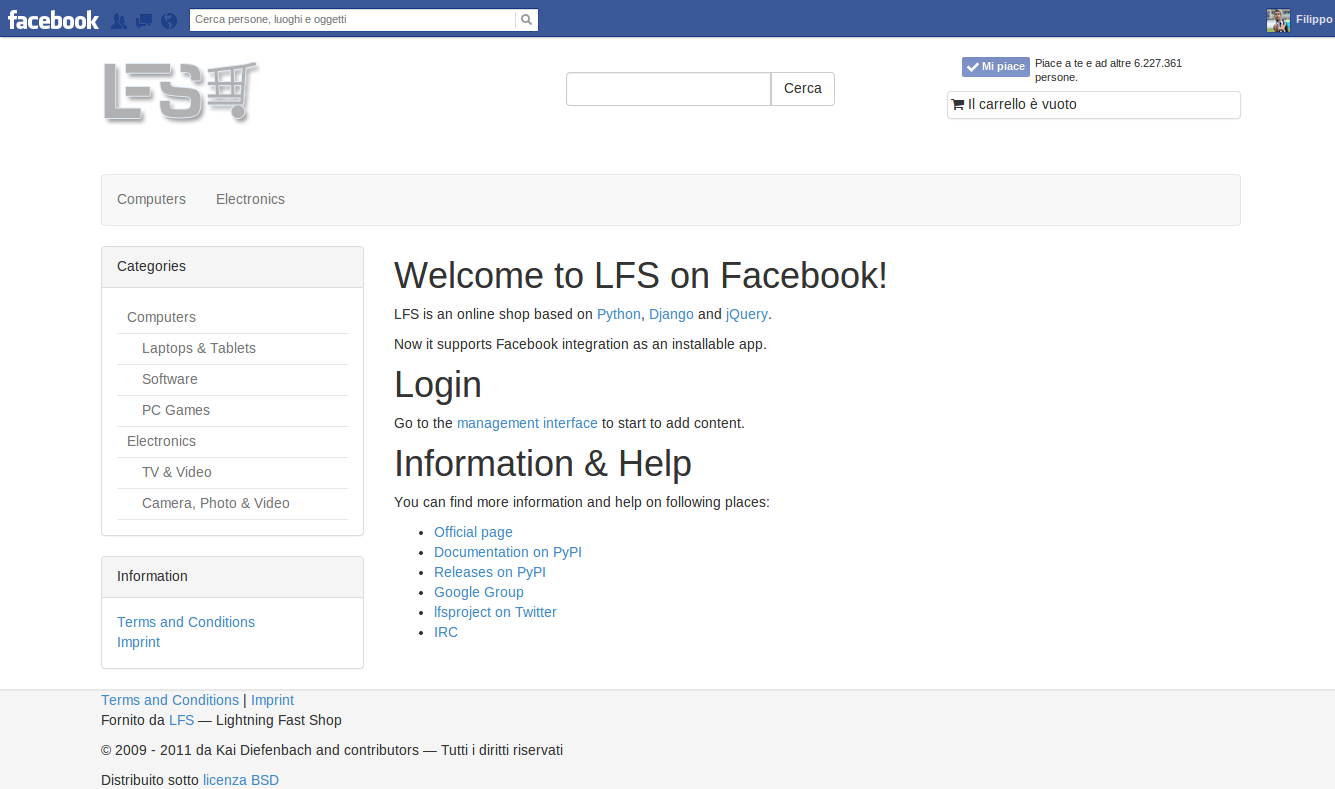
\includegraphics[width=0.9\columnwidth]{img/main_page}
\caption{home page on Facebook}
\end{figure}
Per inserire l'applicazione tra le App di Facebook è necessario procurarsi innanzitutto le credenziali.

Qui i passi utili per ottenerle:
\begin{itemize}
	\item raggiungere la Facebook Developers page\footnote{https://developers.facebook.com/} e autenticarsi con username e password del proprio account facebook;
	\item cliccare su "Create New App";
	\item se non si vede quest'opzione, cliccare su "Register as Developer";
	\item inserire un nome per l'applicazione nel campo "App Name";
	\item accettare le normative della piattaforma Facebook;
	\item inserire il proprio dominio nel campo "App Domains"; poi, portarsi alla sezione "Select how your app integrates with Facebook" e selezionare "Website with Facebook Login." Questa sezione mostrerà un campo "Site URL" dove digitare nuovamente il dominio;
	\item cliccare su "Save Changes".
\end{itemize}
Accedendo alla pagina principale dell'applicazione sono disponibili le due credenziali utili per il proseguo: ID applicazione e App Secret.
Adesso vanno inserite nel file di setting del progetto:

\begin{lstlisting}

FACEBOOK_APP_ID = 'YOUR APP ID'
FACEBOOK_APP_SECRET = 'YOUR APP SECRET NUMBER'

\end{lstlisting}
\begin{figure}
\centering
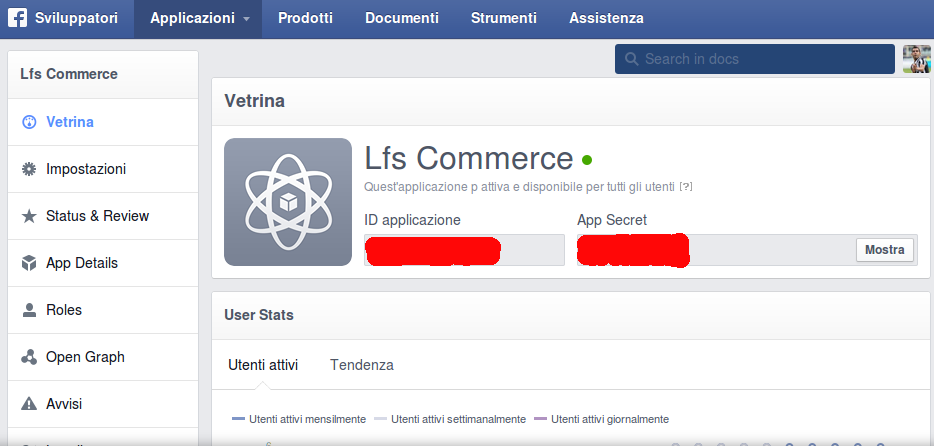
\includegraphics[width=0.9\columnwidth]{img/app_home2}
\caption{basic page for your app}
\end{figure}

%FACEBOOK_CANVAS_PAGE = 'https://apps.facebook.com/%s/' % FACEBOOK_APP_ID

Da notare che è richiesta una connessione https.

\subsection{Facebook plugin}
Facebook fornisce strumenti, servizi ed SDKs per integrare una social experience nelle apps. All'interno delle pagine html di LFS-Facebook si è fatto uso di social plugin il cui codice è fornito agli sviluppatori registrati sulla piattaforma tramite delle pagine nella documentazione che permettono di settare parametri per customizzare il formato dei vari plugin per poi generare il codice di cui fare copy and paste.

Inoltre si sono acquisite delle informazioni del profilo Facebook attraverso delle istruzioni FQL. Facebook Query Language, o FQL, permette di interfacciarci, in modo simile ad SQL, per interrogare i dati ottenuti dalle Graph API.

Le query hanno questa struttura: 
\begin{lstlisting}
SELECT [fields] FROM [table] WHERE [conditions]. 
\end{lstlisting}
Diversamente da SQL la clausola FROM può contenere solo una tabella. Ad ogni query ci si può riferire all'utente loggato attraverso "me()". 

\section{Protezione delle viste con autenticazione richiesta}
L'applicazione si presenta senza un link ad una pagina di login, in quanto l'utente sarà automaticamente rediretto alla procedura di autenticazione quando e se necessario. 

Per ottenere questo comportamento si è scelto di creare un decoratore che protegga le viste desiderate.
Le viste da proteggere non sono imposte dal sistema, ma è tutto pienamente configurabile attravrso il file di setting. Infatti, è stato creato un dizionario di variabili booleane, a ciascuna delle quali corrisponde una pagina che è possibile proteggere settando come 'True' la variabile in questione.


\begin{lstlisting}

VIEW_WITH_LOGIN_REQUIRED = {
    'add-to-cart': True, #True or False
    'shop': False, #True or False
    'category': False, #True or False
    'product': False, #True or False
    'checkout': False, #True or False
}

\end{lstlisting}


Se una vista è protetta da decoratore, sarà dunque scandito l'elenco di variabili: se la variabile corrispondente è uguale a True, sarà chiamato un altro decoratore, nativo del framework Django, @login\textunderscore required, che verificherà lo stato dell'utente, che se loggato procederà verso la pagina richiesta, altrimenti sarà rediretto alla pagina di login.

\begin{lstlisting}

def permissions_required(view_name):
    
    def decorator(func):
        if settings.VIEW_WITH_LOGIN_REQUIRED[view_name]:
            return login_required(func)
        else:
            return func

    return decorator
    
\end{lstlisting}

Comunque si può scegliere di non proteggere alcuna vista e permettere la libera navigazione all'utente che agirà come utente anonimo, potendo aggiungere prodotti al carrello, andare alla cassa, decidere di completare l'acquisto e quindi effettuare il pagamento.

\subsection{Pagina di login}
La pagina di login è stata modificata facendo un override di quella esistente attraverso il linguaggio di template di django, che permette, tra le altre cose, di ereditare da una pagina html e sovrascrivere i blocchi che si vuole.


\begin{lstlisting}[language=html]

 -> inheritance
 -> blocco da sovrascrivere
...


\end{lstlisting}

\begin{figure}
\centering
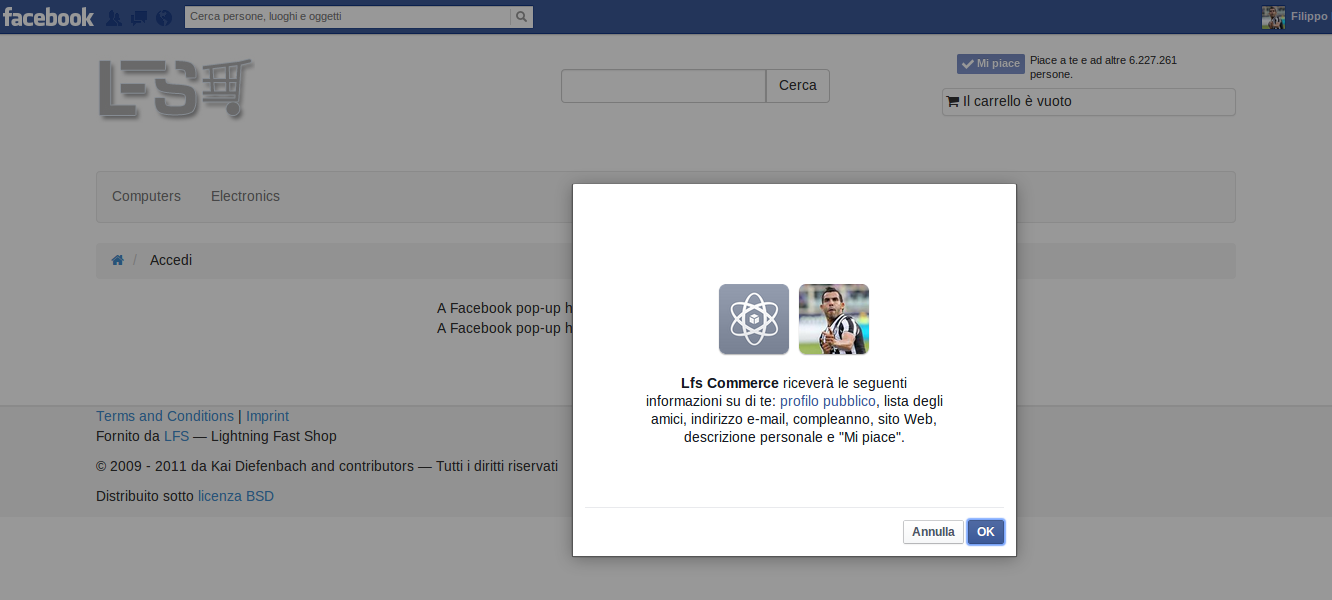
\includegraphics[width=0.9\columnwidth]{img/richiesta_permessi}
\caption{richiesta permessi da parte dell'applicazione}
\end{figure}

Si è scelto di presentare una pagina di login che non richieda nessuna interazione all'utente, infatti l'autenticazione si avvierà in automatico. Per far questo si è utilizzato del codice javascript di django-facebook che effettua il login facebook attraverso le facebook API; il tutto viene scatenato dall'istruzione "F.connect()", ma essendo F una variabile che viene caricata asincronamente, è stato necessario inserire la F.connect all'interno della funzione setInterval (utility di javascript) che prova a chiamare la F.connect ad intervalli di tempo prefissati finchè non avrà successo, ovvero fin quando F non sarà definita. Il meccanismo di chiamata periodica ad uno script verrà fermato attraverso il clearInterval().

\begin{lstlisting}[language=JavaScript]

var myVar = setInterval(function(){
    if(F !== undefined){
        F.connect(document.getElementById('facebook_form'), 
        ['email', 'user_about_me', 'user_birthday', 
        'user_website', 'user_likes']);
        clearInterval(myVar);
    }
    }, 500);

\end{lstlisting}

\subparagraph{template override}
L'override di un template pre-esistente viene effettuato creando un file html con lo stesso identico nome e dovrà essere riprodotta l'alberatura. Per esempio se voglio sovrascrivere lfs/templates/lfs/base.html, dovrò creare un file base.html in myapp/templates/lfs/base.html. 

Dopodichè è necessario anche intervenire nel file di setting ed assicurarsi che fra le INSTALLED\_ APPS, myapp appaia prima della applicazione di cui vogliamo sovrascrivere il template.

\subsection{Pagina di checkout}
La pagina di checkout è l'ultima pagina prima di procedere all'inserimenrto dati per effettuare il pagamento e completare l'acquisto.

Anche di questa pagina è stato fatto un override per visualizzare ancora la possibilità di registrarsi prima dell'acquisto. Se si effettua il login sarà possibile gestire lo stato degli ordini e salvare i dati per prossime spedizioni. Il pulsante del login è un normale elemento html(non un faceboook plugin) il quale stile è stato reso simile a quello Facebook attraverso css. 

\begin{figure}
\centering
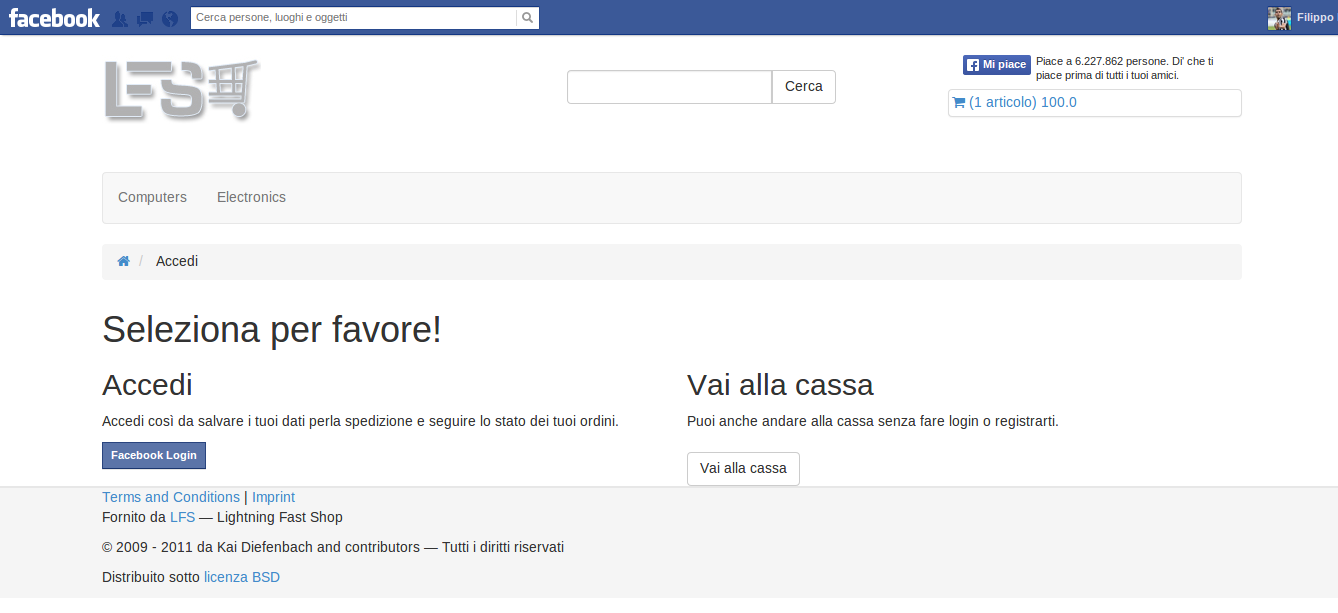
\includegraphics[width=0.9\columnwidth]{img/checkout}
\caption{checkout page}
\end{figure}

\section{Personalizzazione del modello utente}
Il modello è l'unica fonte di informazione a riguardo dei dati che vogliamo memorizzare. Esso contiene i campi e il comportamento per la memorizzazione. 

Quello che vogliamo fare è modificare il modello che definisce la gestione delle informazioni riferite all'utente. Per far questo, si è creato un file models.py, contenente una nuova classe che rappresenta il modello. Questa eredita da FacebookProfileModel la quale è la classe del pacchetto django-facebook che gestiva le informazioni ottenute dal backend di Facebook.

\begin{lstlisting}

class LfsFbUser(FacebookProfileModel):
    user = models.OneToOneField(User)
    fb_like_flag = models.BooleanField(default=False)
	
	...	
	
    class Meta():
            db_table = 'fb_data'
            
\end{lstlisting}

Per settare django affinchè usi il modello appena creato, bisogna modificare il file di setting, aggiungendo infondo al file oppure modificando la voce esistente, in modo da avere:

\begin{lstlisting}

AUTH_PROFILE_MODULE = 'LFS-Facebook.LfsFbUser'

\end{lstlisting}

\section{Prodotti riservati ai fan}
Come feature aggiuntiva si è pensato di dare la possibilità a chi mette in piedi l'e-commerce, di poter riservare l'acquisto di un prodotto soltanto chi è un Facebook fan, ovvero a chi ha messo il "mi piace" alla pagina Facebook del negozio.

Per far ciò bisogna connfigurare il sistema specificando l'identificativo della pagina facebook nel solito file di setting, come segue:
%\begin{figure}
%
%\end{figure}

\begin{lstlisting}

FACEBOOK_PAGE = 'YOUR PAGE ID'

\end{lstlisting}

Per distinguere un prodotto riservato ai fan, si utilizza una zaratteristica di LFS che sono le "PROPRIETA". queste si possono gestire da web, loggandosi attraverso un utente amminstratore ed entrando nella sezione gestione del sito. Cosa importante è il titolo della proprietà, in quanto questo attributo verrà poi utilizzato nel codice.

\begin{lstlisting}

fb_reserved = "False"
    for p in product.get_properties():
        if p.title == settings.FACEBOOK_FAN_RESERVED_PROPERTY:
            fb_reserved = "True"
            
\end{lstlisting}

Il titolo da adottare è settabile anch'esso nel setting.py:

\begin{lstlisting}

FACEBOOK_FAN_RESERVED_PROPERTY = "YOUR PROPERTY TITLE"

\end{lstlisting}

Trovate le modalità per marcare un prodotto come riservato, è importante vedere come controllare se l'utente soddisfa i requisiti per effettuare l'acquisto.

Per far questo si è ricorso ad una FQL Query che selezione un user ID se ha tra i propri mi piace alle pagine, quello ricercato.

\begin{lstlisting}

var fql_query = "SELECT uid 
		FROM page_fan 
		WHERE page_id = "+fbPage+
		" and uid = "+user_id;
				
\end{lstlisting}

nota: Per effettuare questa query è necessario aver richiesto i permessi in fase di login. 

Attraverso una Facebook API, eseguiamo la query, e ci muoviamo di conesguenza; in particolare, attraverso jQuery, se l'utente è abilitato all'acquisto, si abilita il pulsante di aggiunta al carrello e si mostra un determinato messaggio, altrimenti si disibalita il pulsante e si mostra un messaggio complementare.
\begin{figure}
\centering
\subfigure[no reserved product]
	{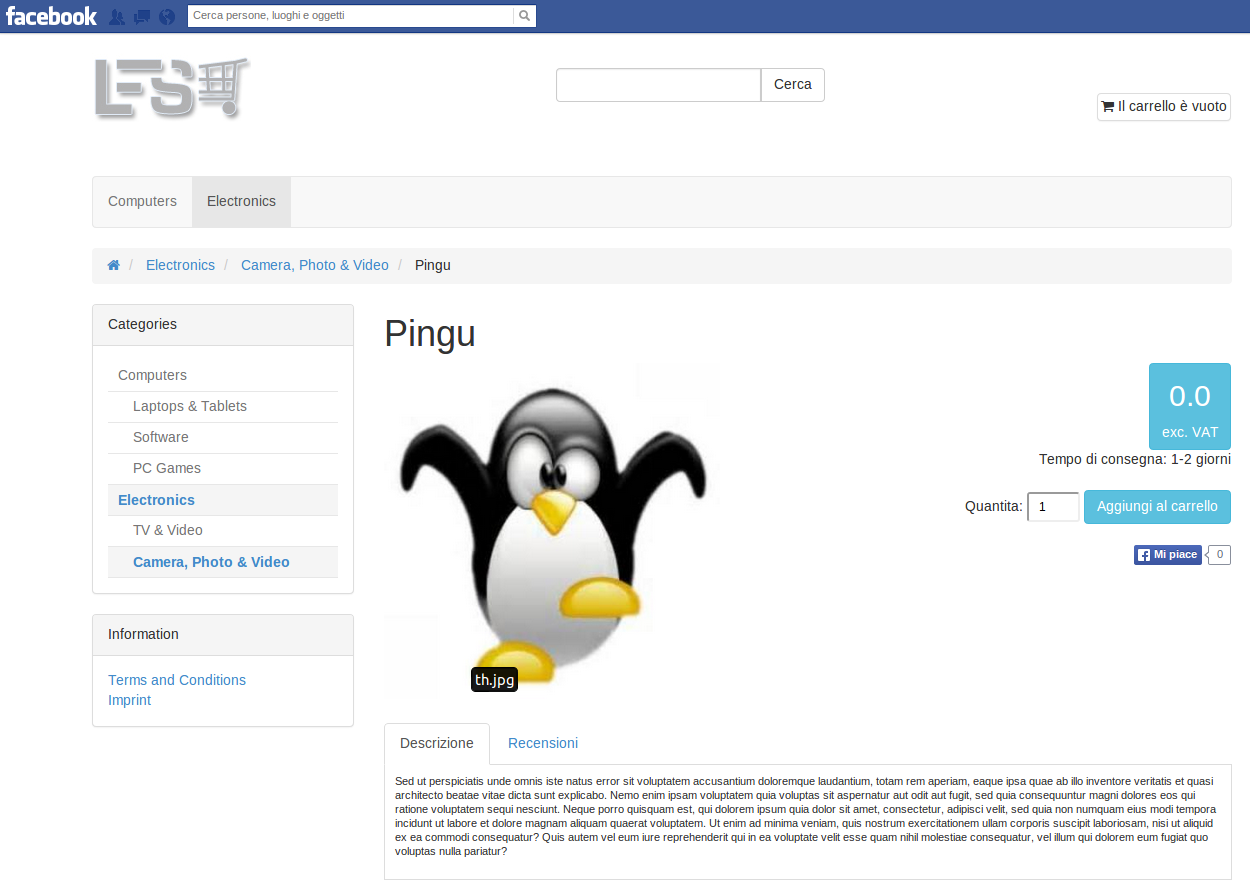
\includegraphics[width=0.9\columnwidth]
	{img/product_view}}
\subfigure[Facebook fan]
	{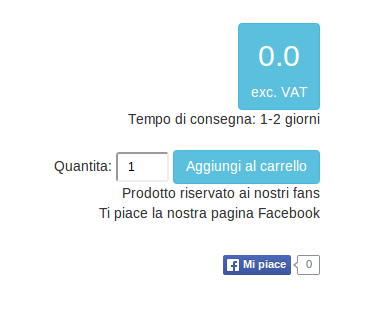
\includegraphics[width=0.4\columnwidth]{img/detail_product_view_fb_reserved}}
\hspace{5mm}
\subfigure[no Facebook fan]
	{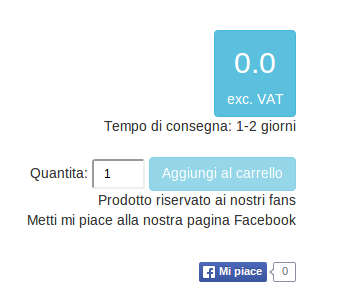
\includegraphics[width=0.4\columnwidth]{img/detail_product_view_no_fan}}
\caption{product view}
\end{figure}
\begin{lstlisting}

    $(document).ready(FB.api({
        method: 'fql.query',
        query: fql_query
    },
    function(response){
        if(fbReserved == "True"){
            if (response.length == 1 && response[0].uid == user_id){
                allowPurchase(true);
            } else {
                allowPurchase(false);
            }
        }else{
            $("#add-to-cart").prop('disabled', false);

            $("#fb-no-like").hide();
            $("#fb-already-like").hide();
        }
    }));

\end{lstlisting}

\section{Internazionalizzazione}
Lo sviluppo di un’applicazione web richiede, sempre più frequentemente, di potere essere utilizzata da una moltitudine di utenti di lingue e culture diverse.

La soluzione a questa esigenza è di consentire a questi utenti di poter scegliere la lingua con cui desiderano navigare le pagine dell’applicazione stessa.

L'internazionalizzazione è il processo mediante il quale vengono eliminati dal codice sorgente i preconcetti culturali quali il formato della data, la formattazione dei numeri, la visualizzazione di immagini raffiguranti elementi tipici di un determinato paese (autobus, cassette della posta, ecc.). 

La Localizzazione è il processo di adattamento di un’applicazione per permetterle di poter cambiare dinamicamente le risorse presenti nelle pagine: principalmente stringhe ma anche file di testo, immagini, file audio e ogni altro tipo di contenuto inseribile in una pagina web.
Quindi codice del tipo:

lblMessaggio.Text = “Ciao Mondo!”

deve essere riscritto in modo che la stringa “Ciao Mondo!” non sia statica, ma possa variare in modalità runtime secondo la lingua scelta dall’utente.

Django supporta pienamente la traduzione del testo, formattazione delle date, orari, numeri e  time zones.

Questo viene fatto essenzialmente attraverso due passi:
\begin{itemize}
	\item si specificano quali parti della propria app dovrebbero essere tradotte o formattate per culture e/o lingue specifiche;
	\item django usa questi "ganci" per localizzare la Web app per un utente specifico secondo le proprie impostazioni.
\end{itemize}

La parola 'Internationalization' è spesso abbreviata con 'i18n'. Questa abbreviazione è largamente usata, deriva dal fatto che ci sono 18 lettere tra la 'i' e la 'n'.

Sebbene il meccanismo di traduzione può essere avviato da molti tipi di file, per esempio nel codice python, javascript, etc... per il nostro lavoro è stato sufficiente supportare l'internazionalizzazione nell'html. Più in dettaglio, in testa alle pagine desiderate, in accordo con il linguaggio django, è stato inserito  il tag
\begin{lstlisting}

\end{lstlisting}
ed ogni elemento di cui si disporrà di una traduzione va inserito tra il tag \begin{lstlisting}

\end{lstlisting}
Successivamente è stato necessario scrivere la traduzione. Per far questo si utilizza il comando
\begin{lstlisting}
django-admin.py makemessages -l <id_language>
\end{lstlisting}
il quale crea un file con l'elenco delle voci da tradurre e la giusta alberatura  nel quale inserirlo. Ovviamente adesso va qui inserita la traduzione frase per frase. Successivamente lanciando il comando 
\begin{lstlisting}
<django-admin.py compilemessages>
\end{lstlisting}
verrà creato il file di estensione .mo utilizzato dal sistema per le traduzioni.

\endinput
